%%%%%%%%%%%%%%%%%%%%%%%%%%%%%%%%%%%%%%%%%
% University/School Laboratory Report
% LaTeX Template
% Version 3.1 (25/3/14)
%
% This template has been downloaded from:
% http://www.LaTeXTemplates.com
%
% Original author:
% Linux and Unix Users Group at Virginia Tech Wiki 
% (https://vtluug.org/wiki/Example_LaTeX_chem_lab_report)
%
% License:
% CC BY-NC-SA 3.0 (http://creativecommons.org/licenses/by-nc-sa/3.0/)
%
%%%%%%%%%%%%%%%%%%%%%%%%%%%%%%%%%%%%%%%%%

%----------------------------------------------------------------------------------------
%	PACKAGES AND DOCUMENT CONFIGURATIONS
%----------------------------------------------------------------------------------------

\documentclass{article}

\usepackage[version=3]{mhchem} % Package for chemical equation typesetting
\usepackage{siunitx} % Provides the \SI{}{} and \si{} command for typesetting SI units
\usepackage{graphicx} % Required for the inclusion of images
\usepackage{natbib} % Required to change bibliography style to APA
\usepackage{amsmath} % Required for some math elements 

\setlength\parindent{0pt} % Removes all indentation from paragraphs

\renewcommand{\labelenumi}{\alph{enumi}.} % Make numbering in the enumerate environment by letter rather than number (e.g. section 6)

%\usepackage{times} % Uncomment to use the Times New Roman font

%----------------------------------------------------------------------------------------
%	DOCUMENT INFORMATION
%----------------------------------------------------------------------------------------

\title{EPICS UPRC \\ Week 3 \\ RFID - Tech team} % Title


\date{\today} % Date for the report

\begin{document}

\maketitle % Insert the title, author and date

% If you wish to include an abstract, uncomment the lines below
% \begin{abstract}
% Abstract text
% \end{abstract}

%----------------------------------------------------------------------------------------
%	SECTION 1
%----------------------------------------------------------------------------------------

\section{Progress}
	\begin{itemize}
	\item Set up a Github repository to host the code
  \item Did a small experiment to make sure Arduino works\\
  	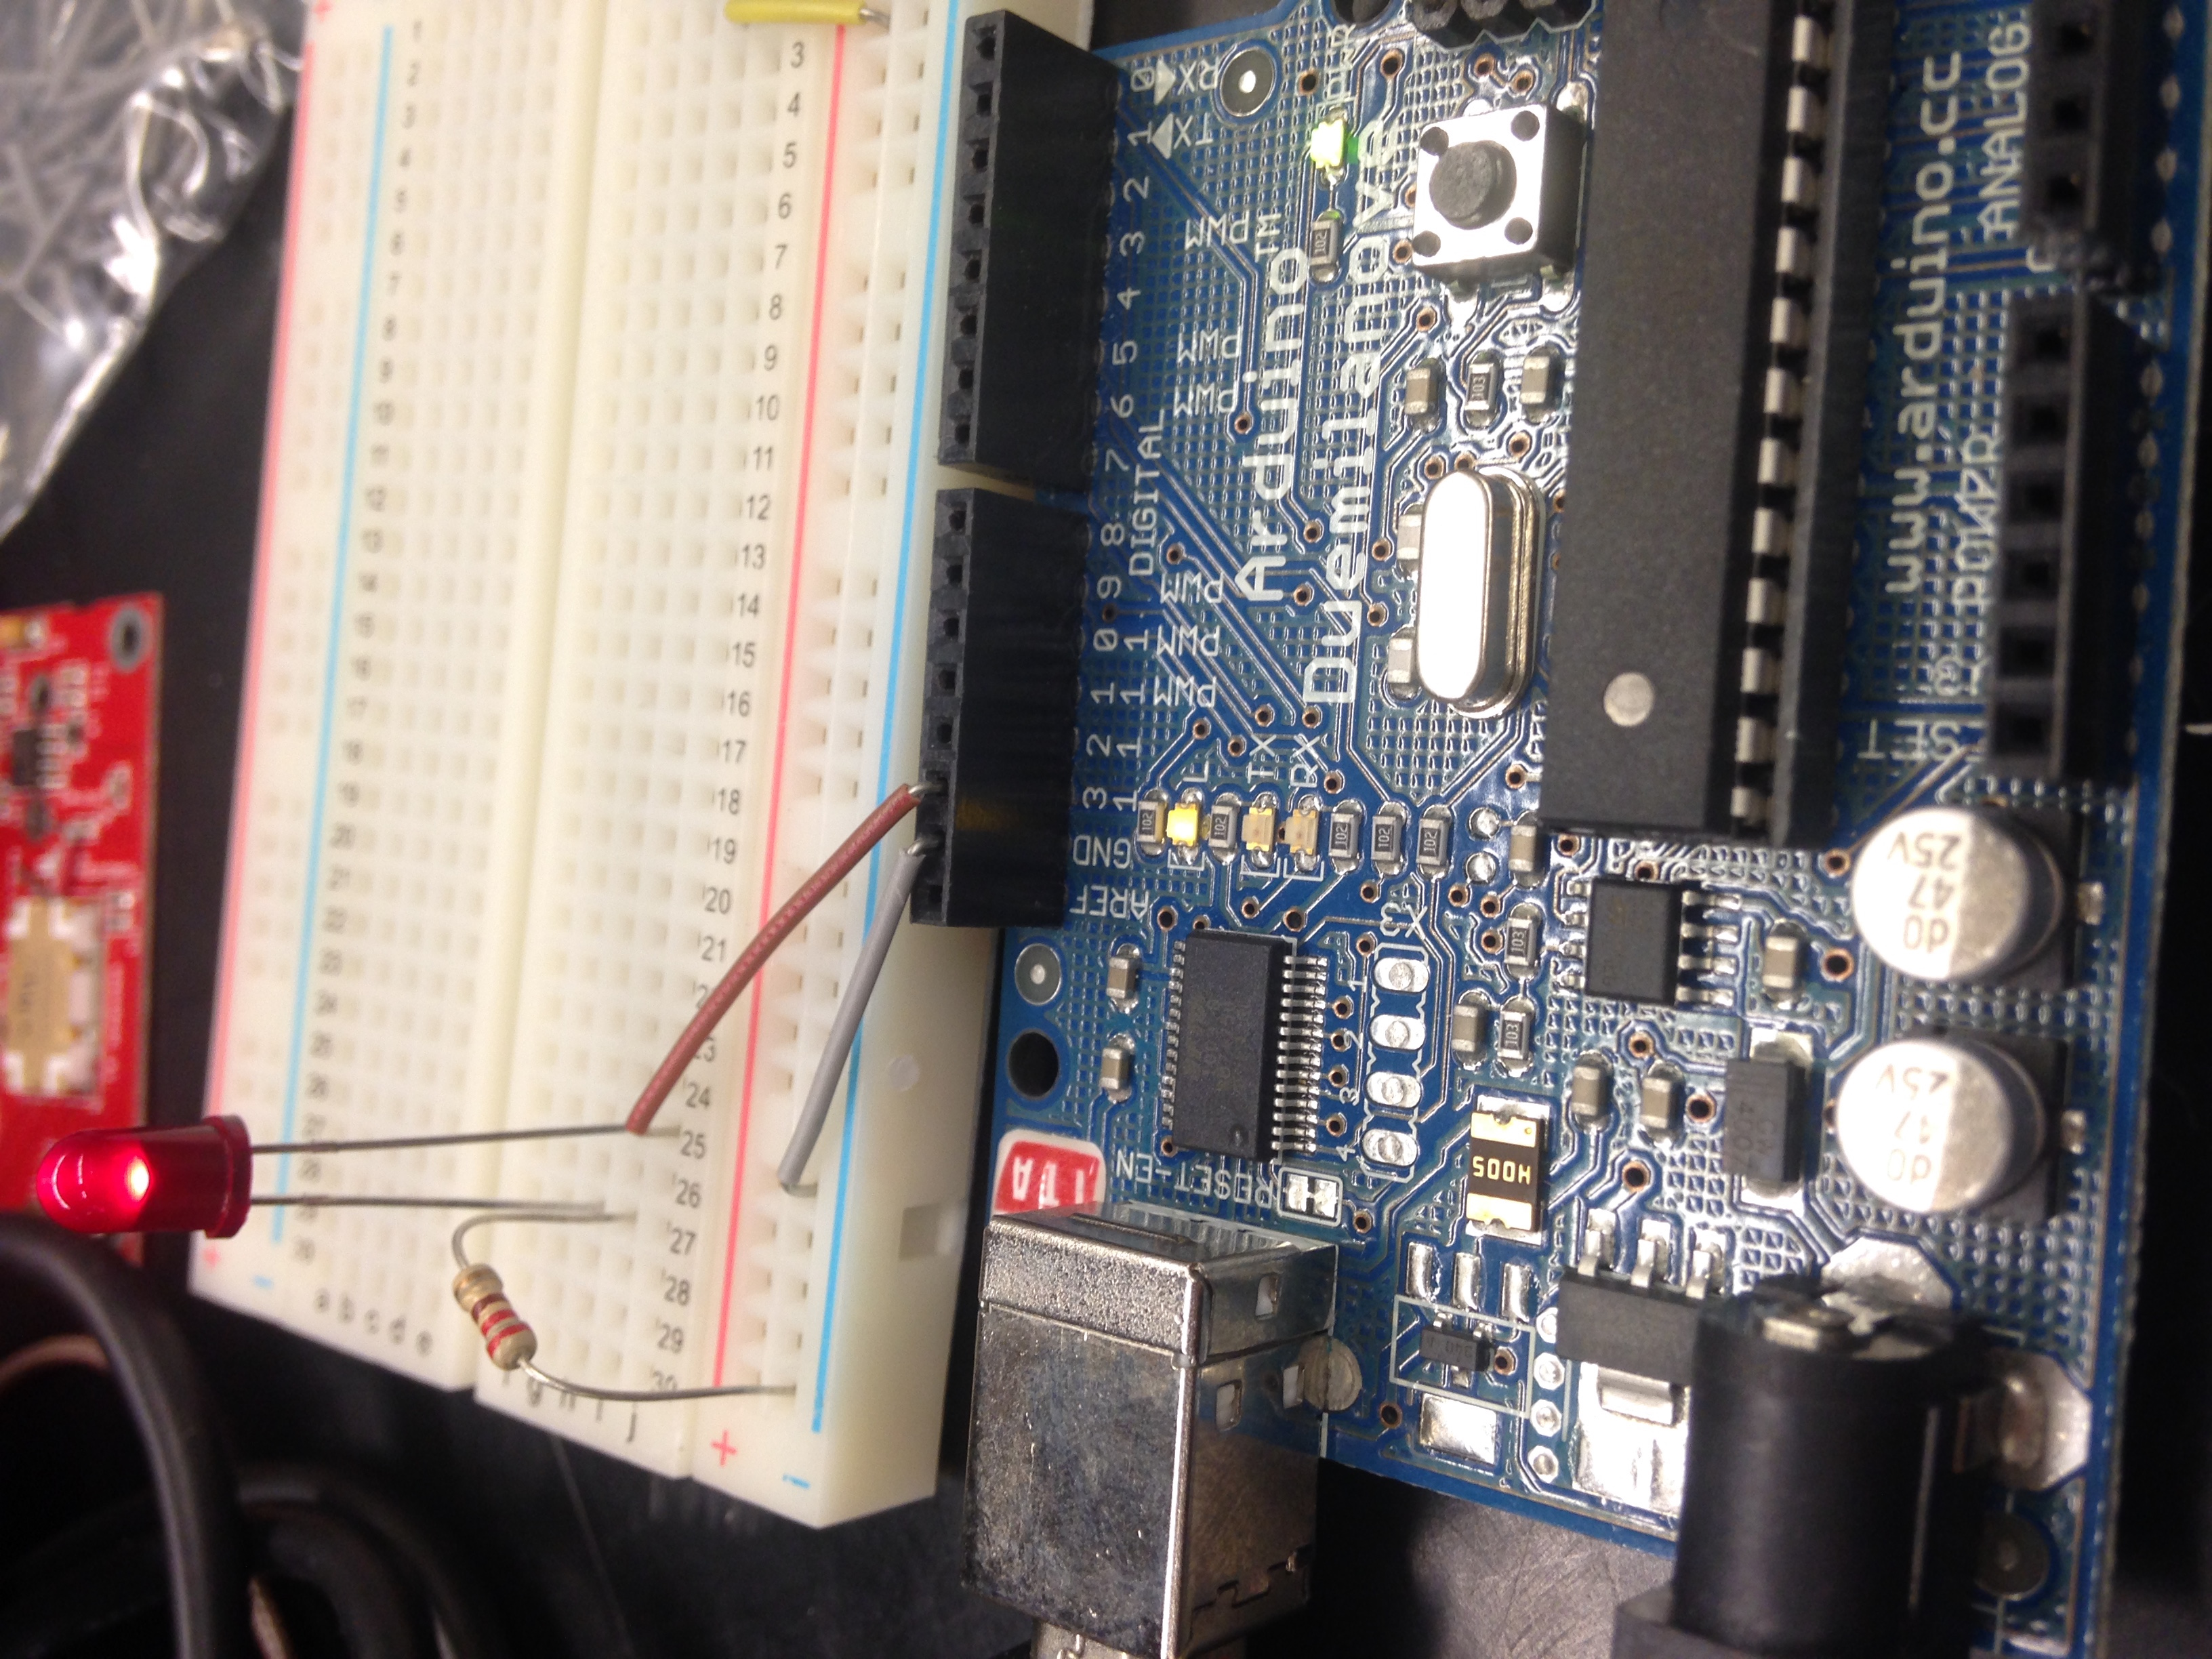
\includegraphics[scale=0.09,angle=-90]{works.JPG} 
  
  \item Tried setting up Arduino, the reader and antenna. \\
   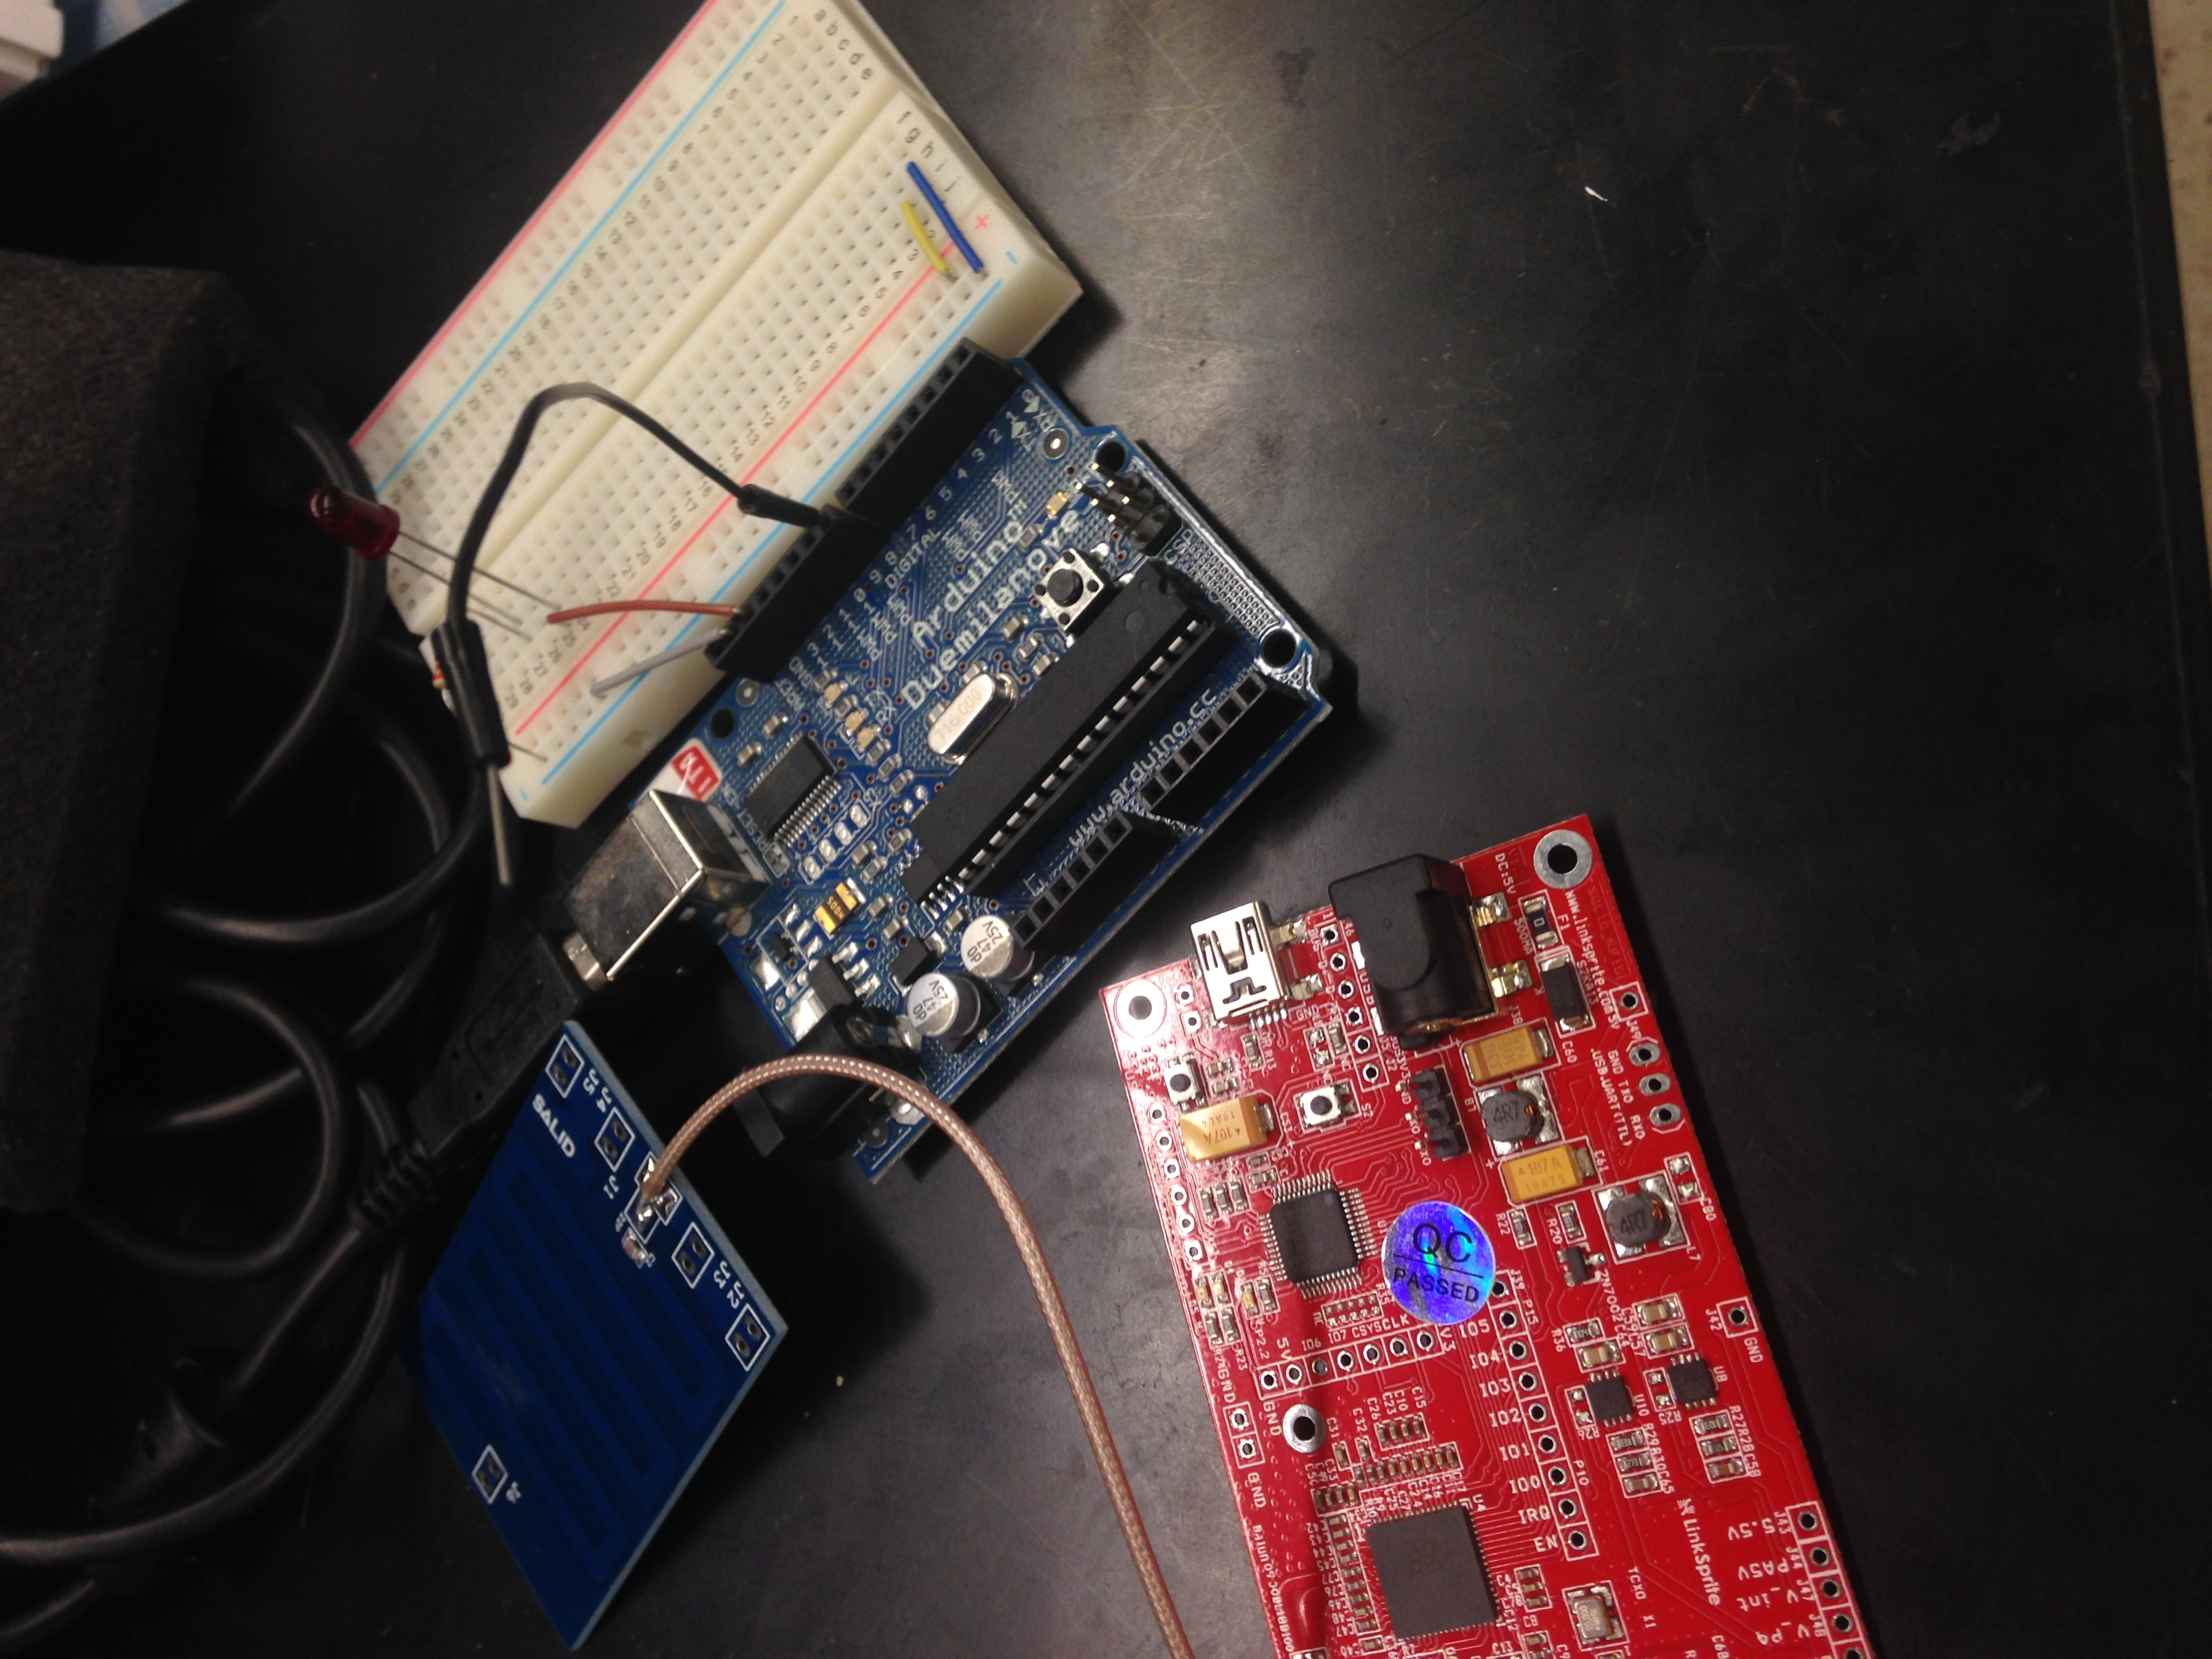
\includegraphics[scale=0.1,angle=-90]{IMG_2848.JPG} 
\end{itemize}

\section{Issues}
\begin{itemize}
\item Can't find the jumper wire
\item Andrew fooled me by using a wrong case on the Arduino \\
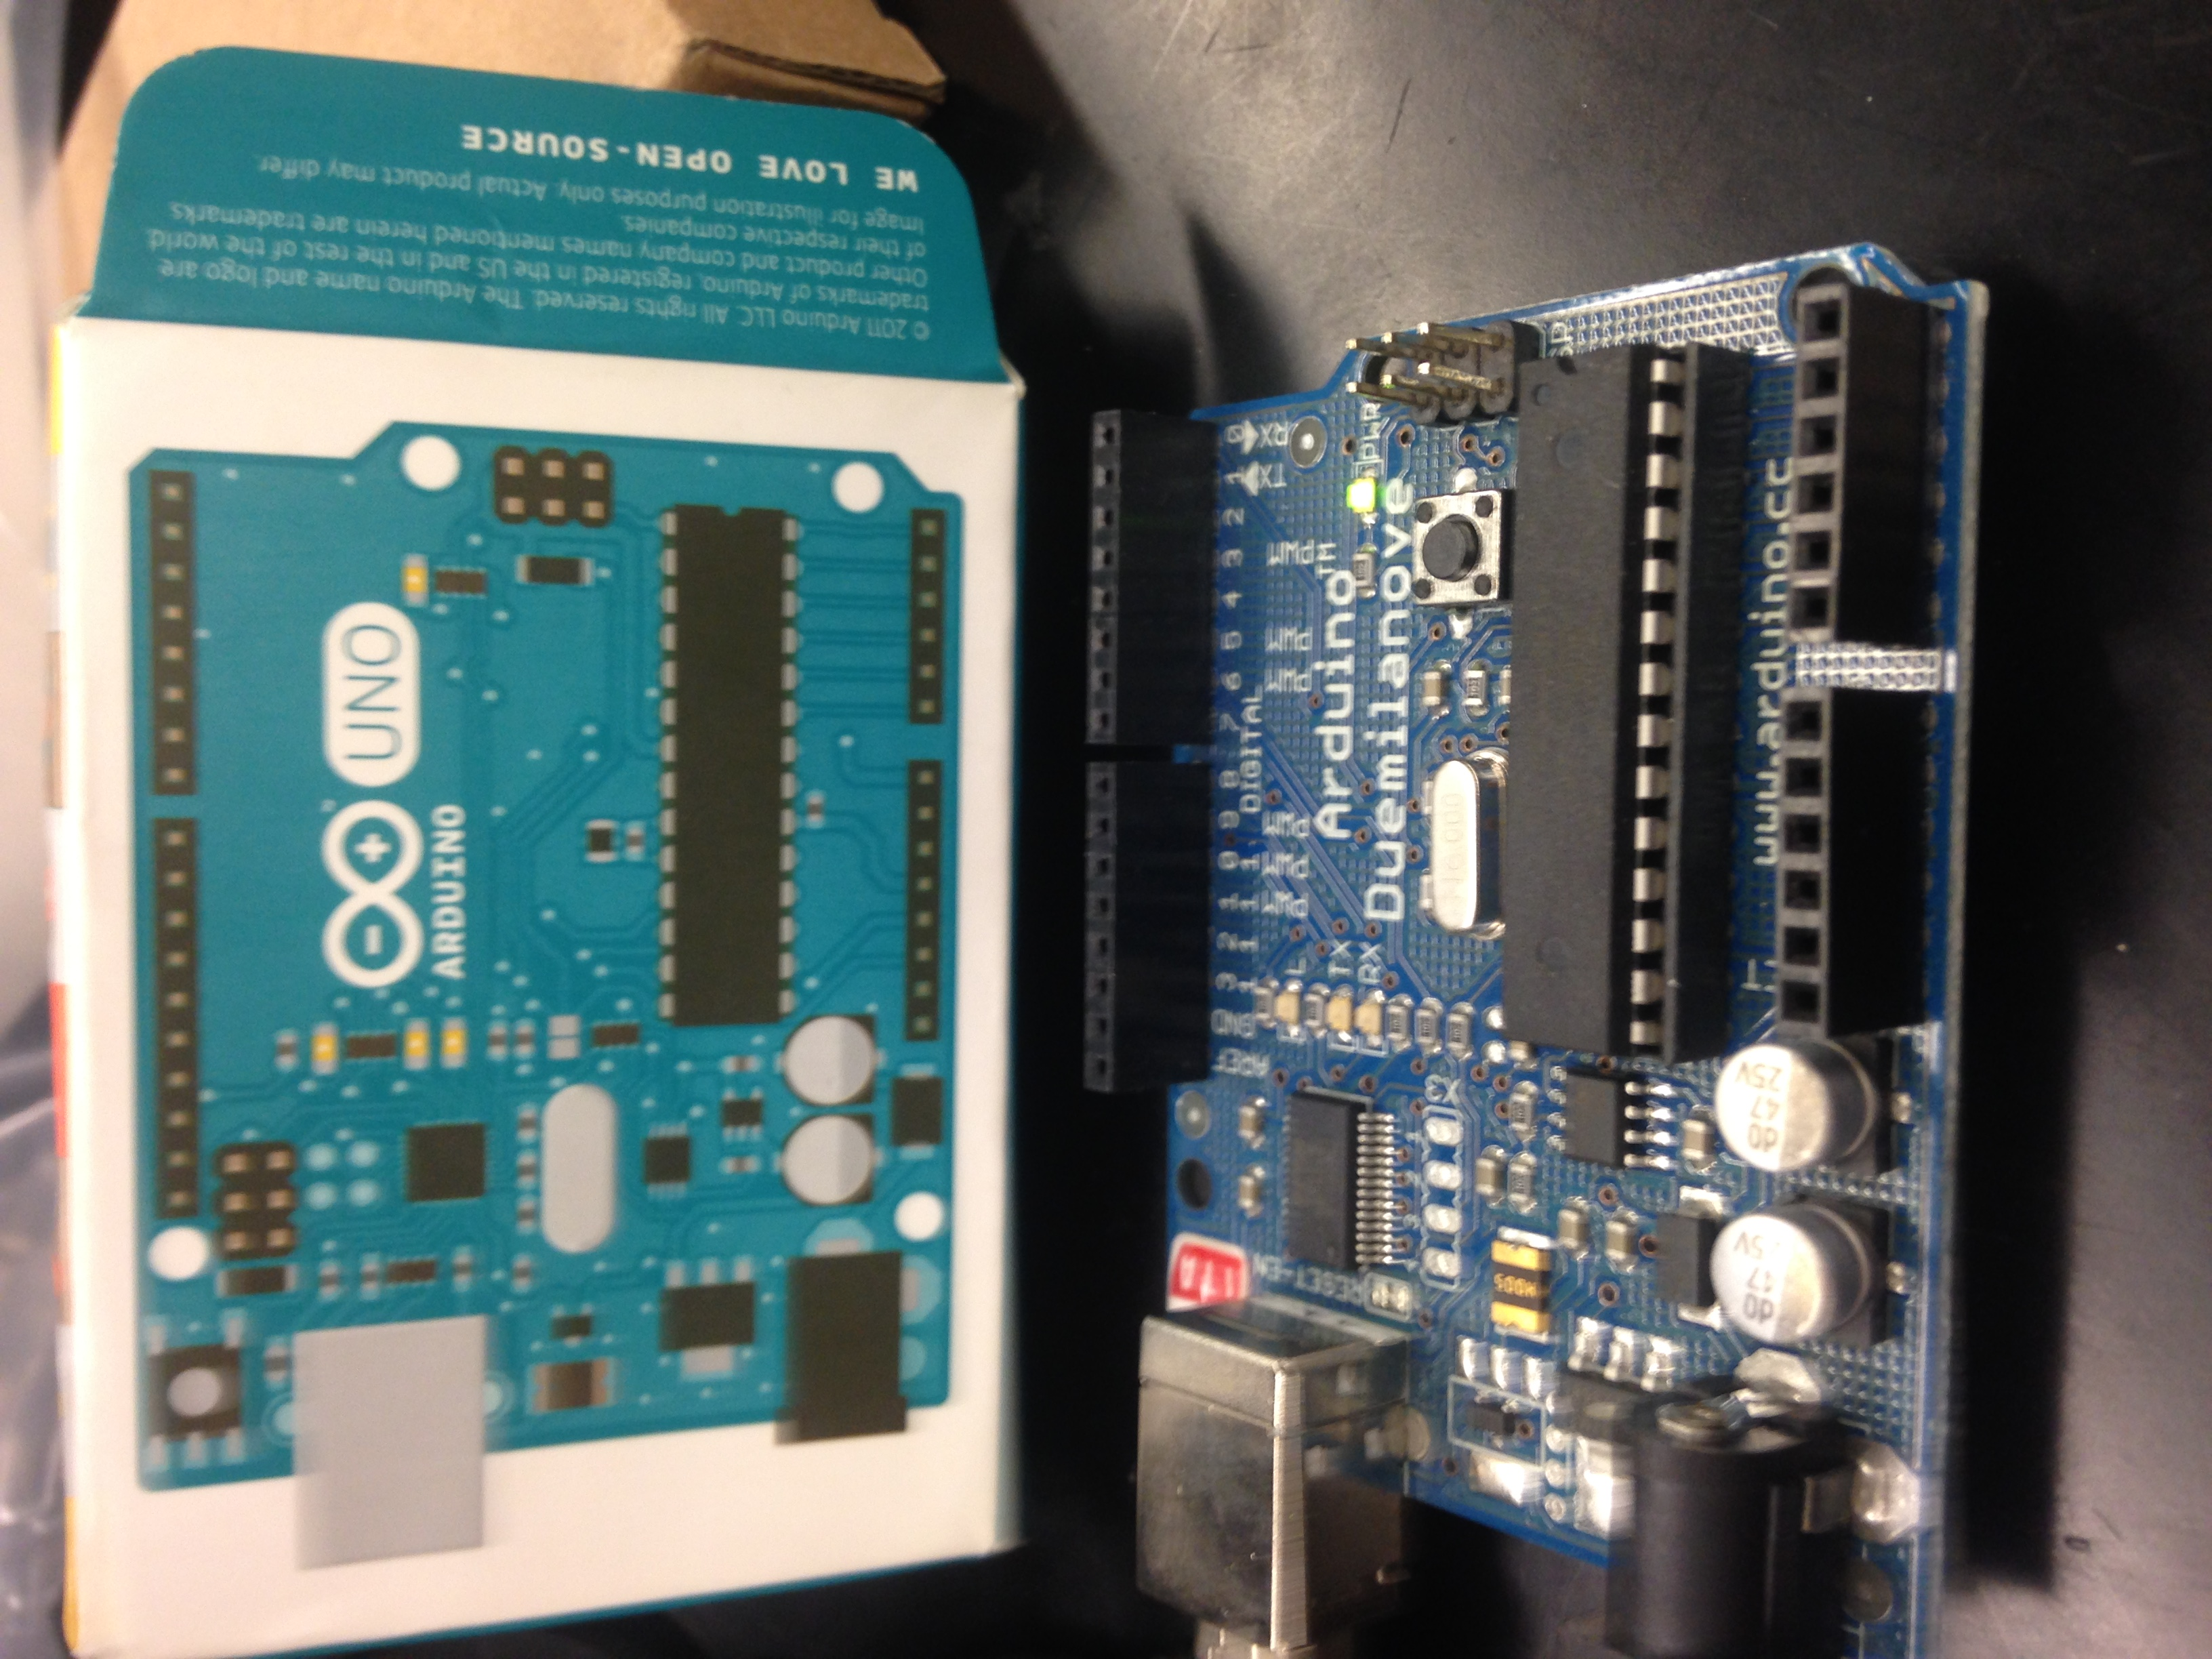
\includegraphics[scale=0.1,angle=-90]{IMG_2845.JPG} 
\end{itemize}
\section{Goals}
\begin{itemize}
\item Continue setting up the hardware
\item Start coding the Arduino
\end{itemize}

%----------------------------------------------------------------------------------------


\end{document}